% !TEX root = trkjet.tex

The \Dptr\ distributions are studied as a function of \ptjet\ for \pp\ data and \PbPb\ collisions with different centralities.
The interplay between the hot and dense matter and the parton shower is explored by evaluating the ratios and differences between \Dptr\ distributions in \pbpb\ and \pp\ collisions, as well as some integrated quantities.



%%%%%%%    DPtr distributions    %%%%%%%
\subsection{\Dptr\ distributions}
\label{sec:dptr}
The \Dptr\ distributions evaluated in \pp\ and \pbpb\ collisions for $126 < \ptjet < 158$ GeV are shown in Figure~\ref{fig:dptr}.
The distributions exhibit a difference in shape between \PbPb\ and \pp\ collisions, with the \pbpb\ distributions being broader at low \pt\ (\pt < 4 GeV) and narrower at high \pt\ (\pt > 4 GeV) in \mbox{0--10\%} central collisions.
This modification is centrality dependent and is smaller for peripheral \pbpb\ collisions.

\begin{figure}[h]
\centerline{
\begin{tabular}{ccc}
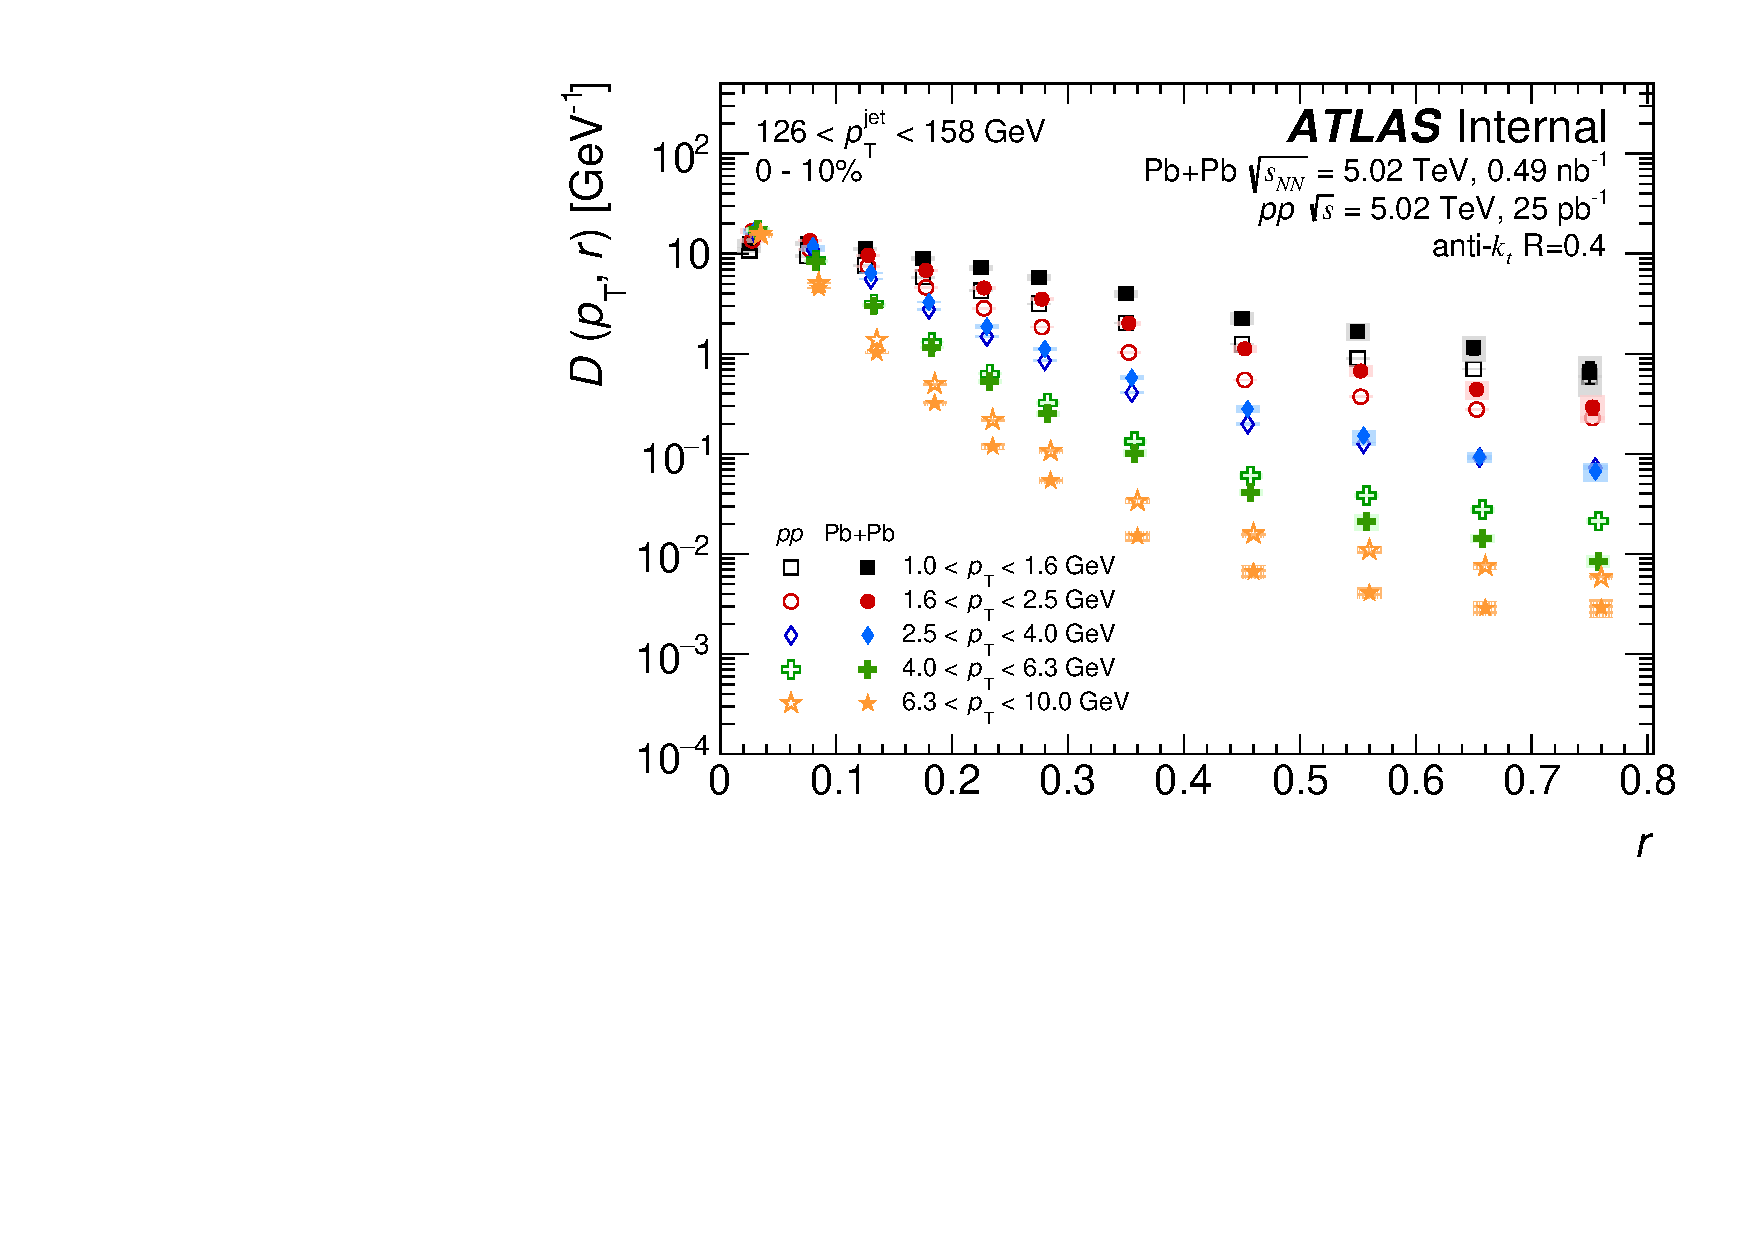
\includegraphics[width=0.36\textwidth]{figures/results/DpT_dR_jet7_cent0} &
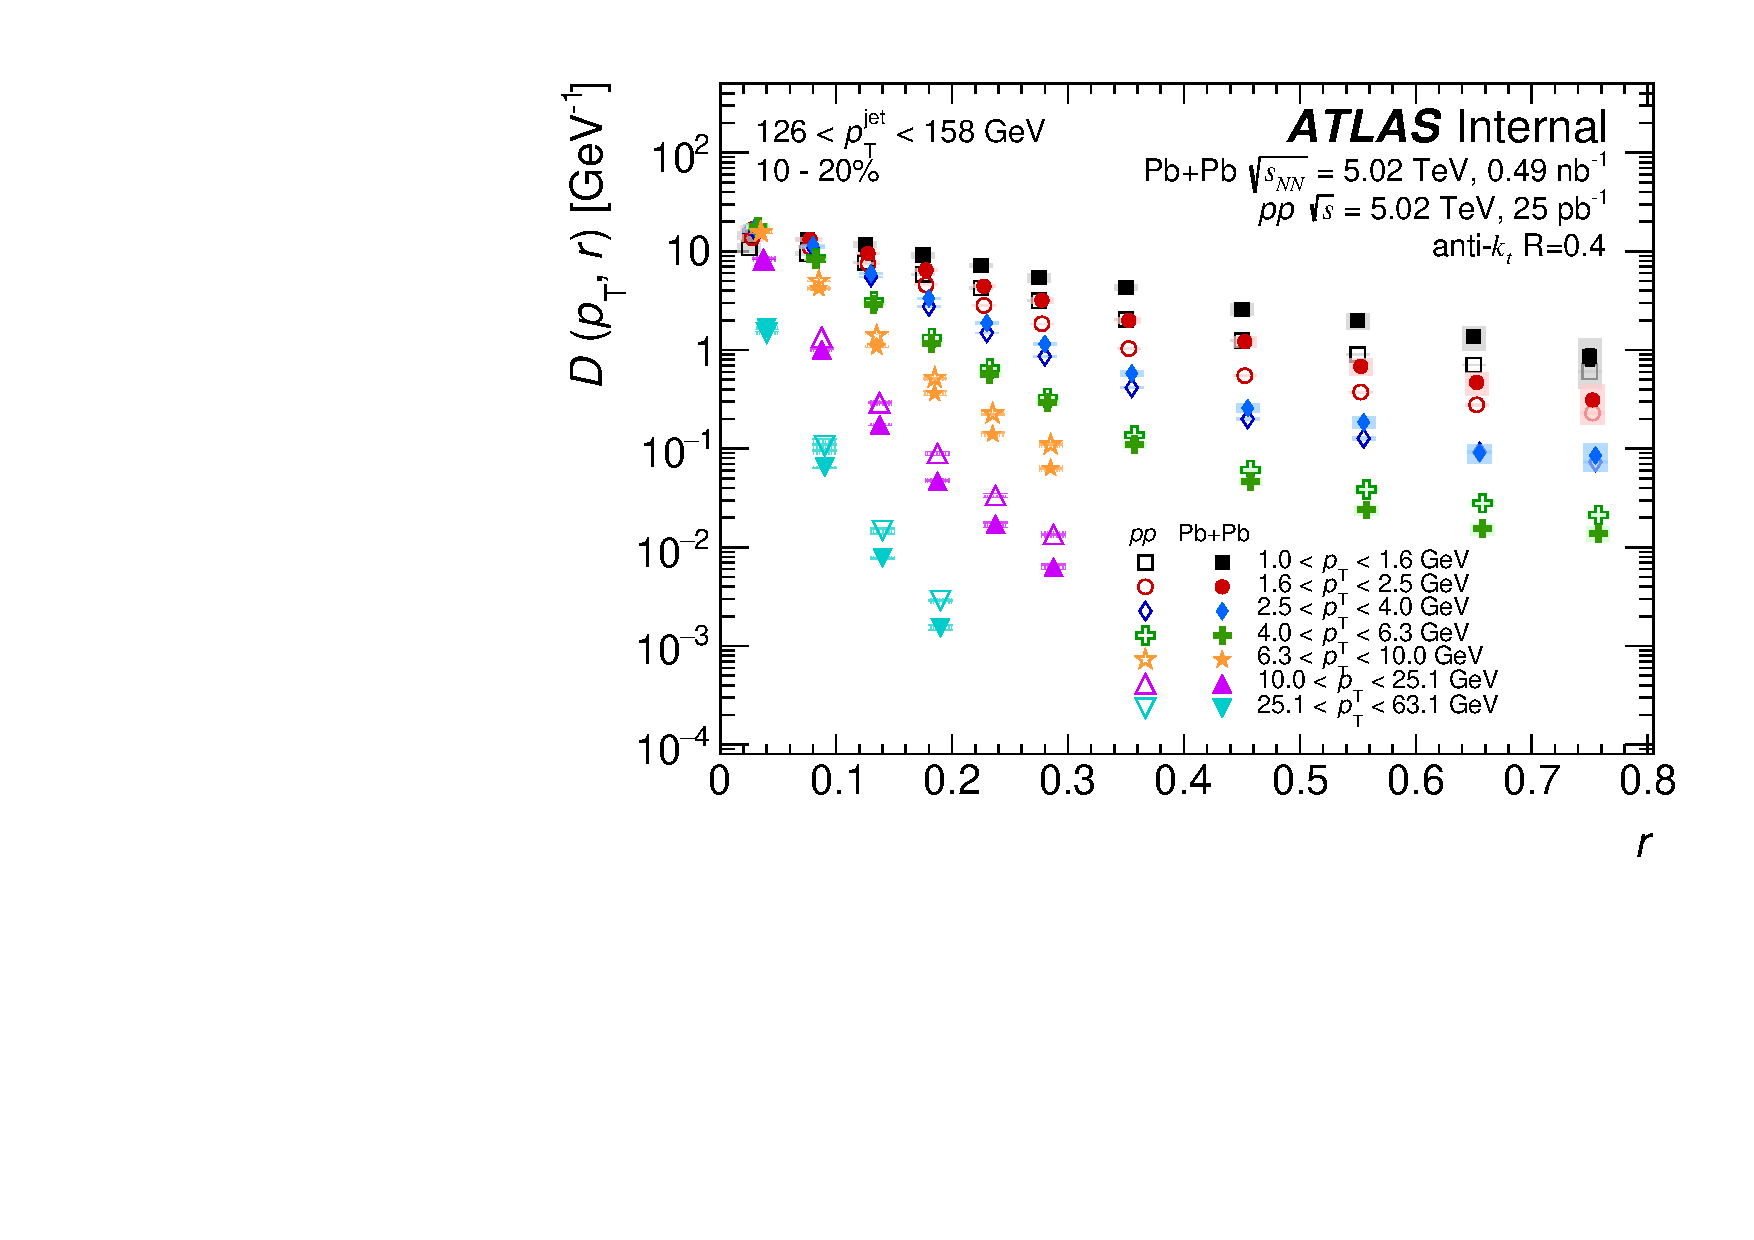
\includegraphics[width=0.36\textwidth]{figures/results/DpT_dR_jet7_cent1} &
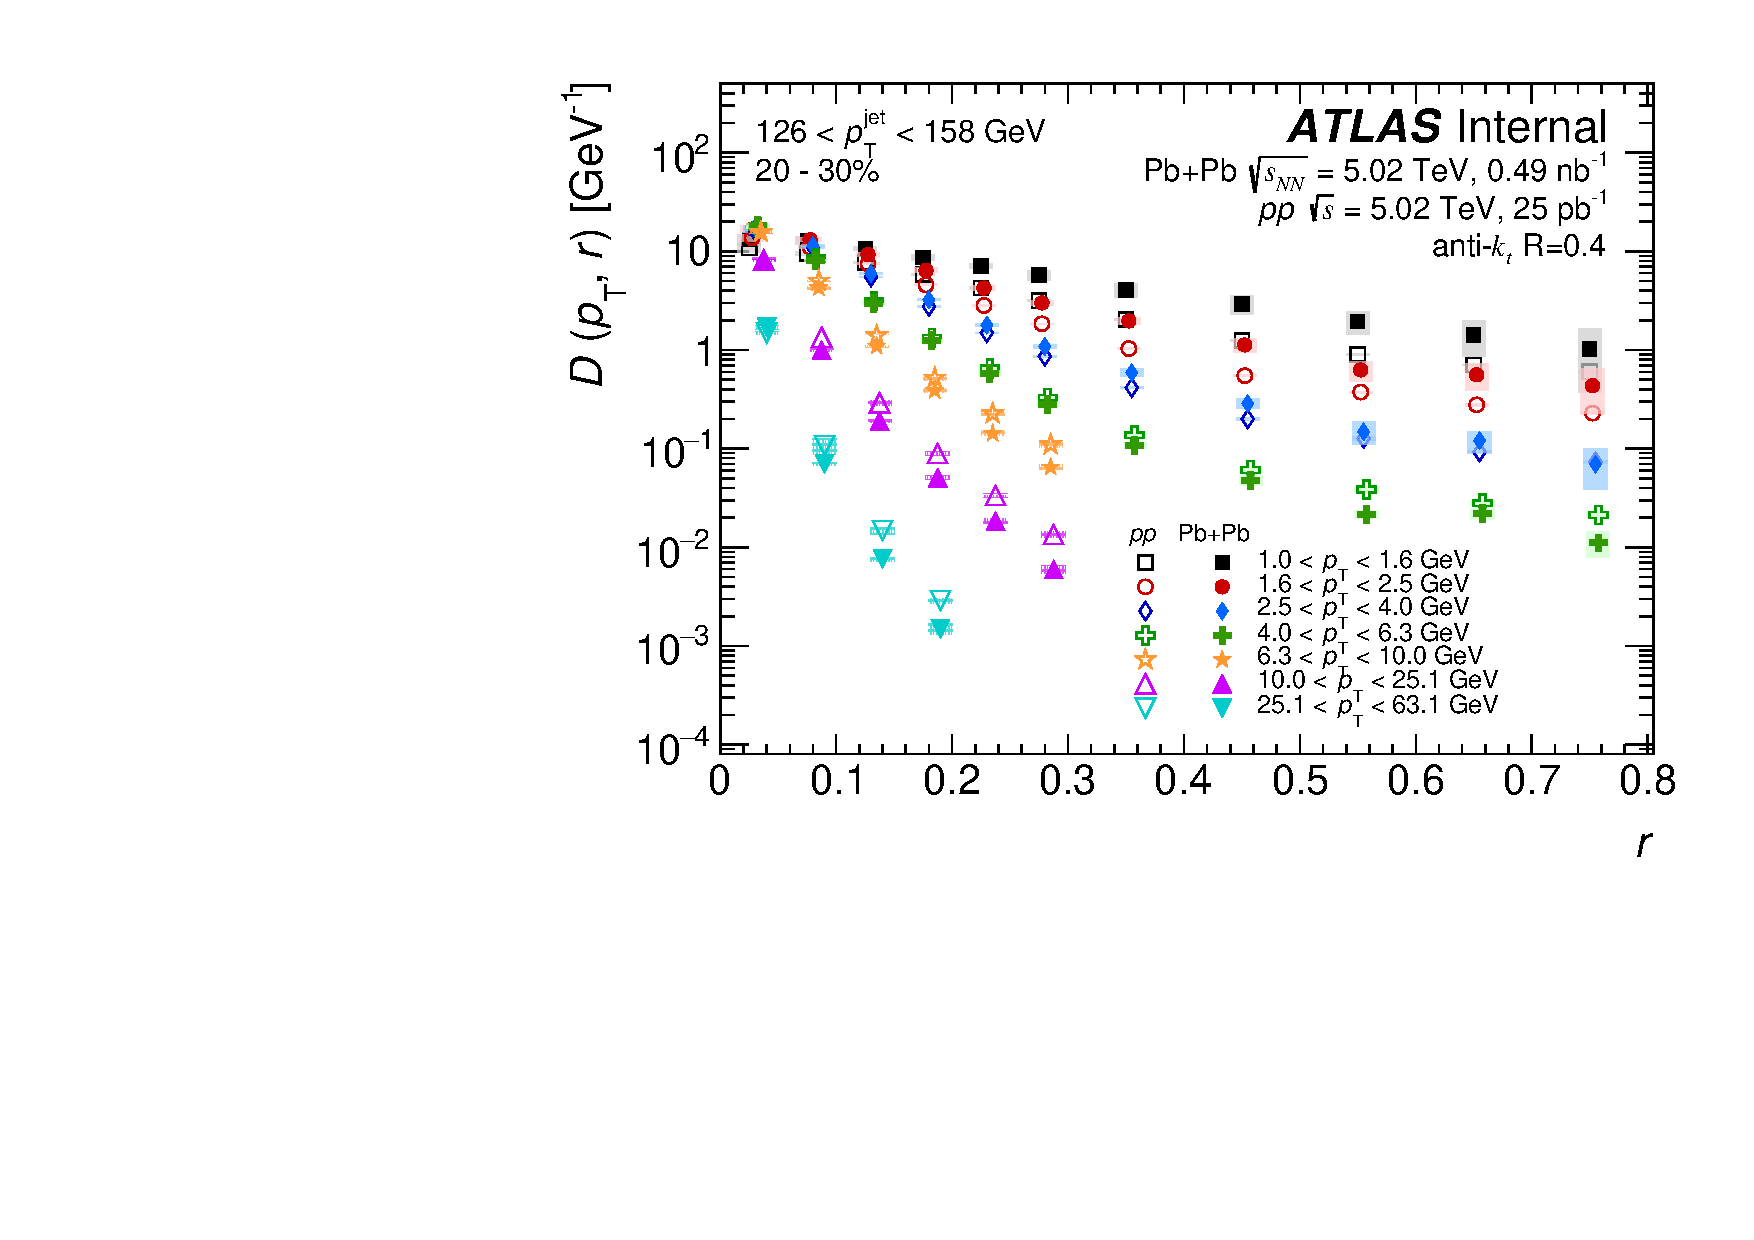
\includegraphics[width=0.36\textwidth]{figures/results/DpT_dR_jet7_cent2} \\
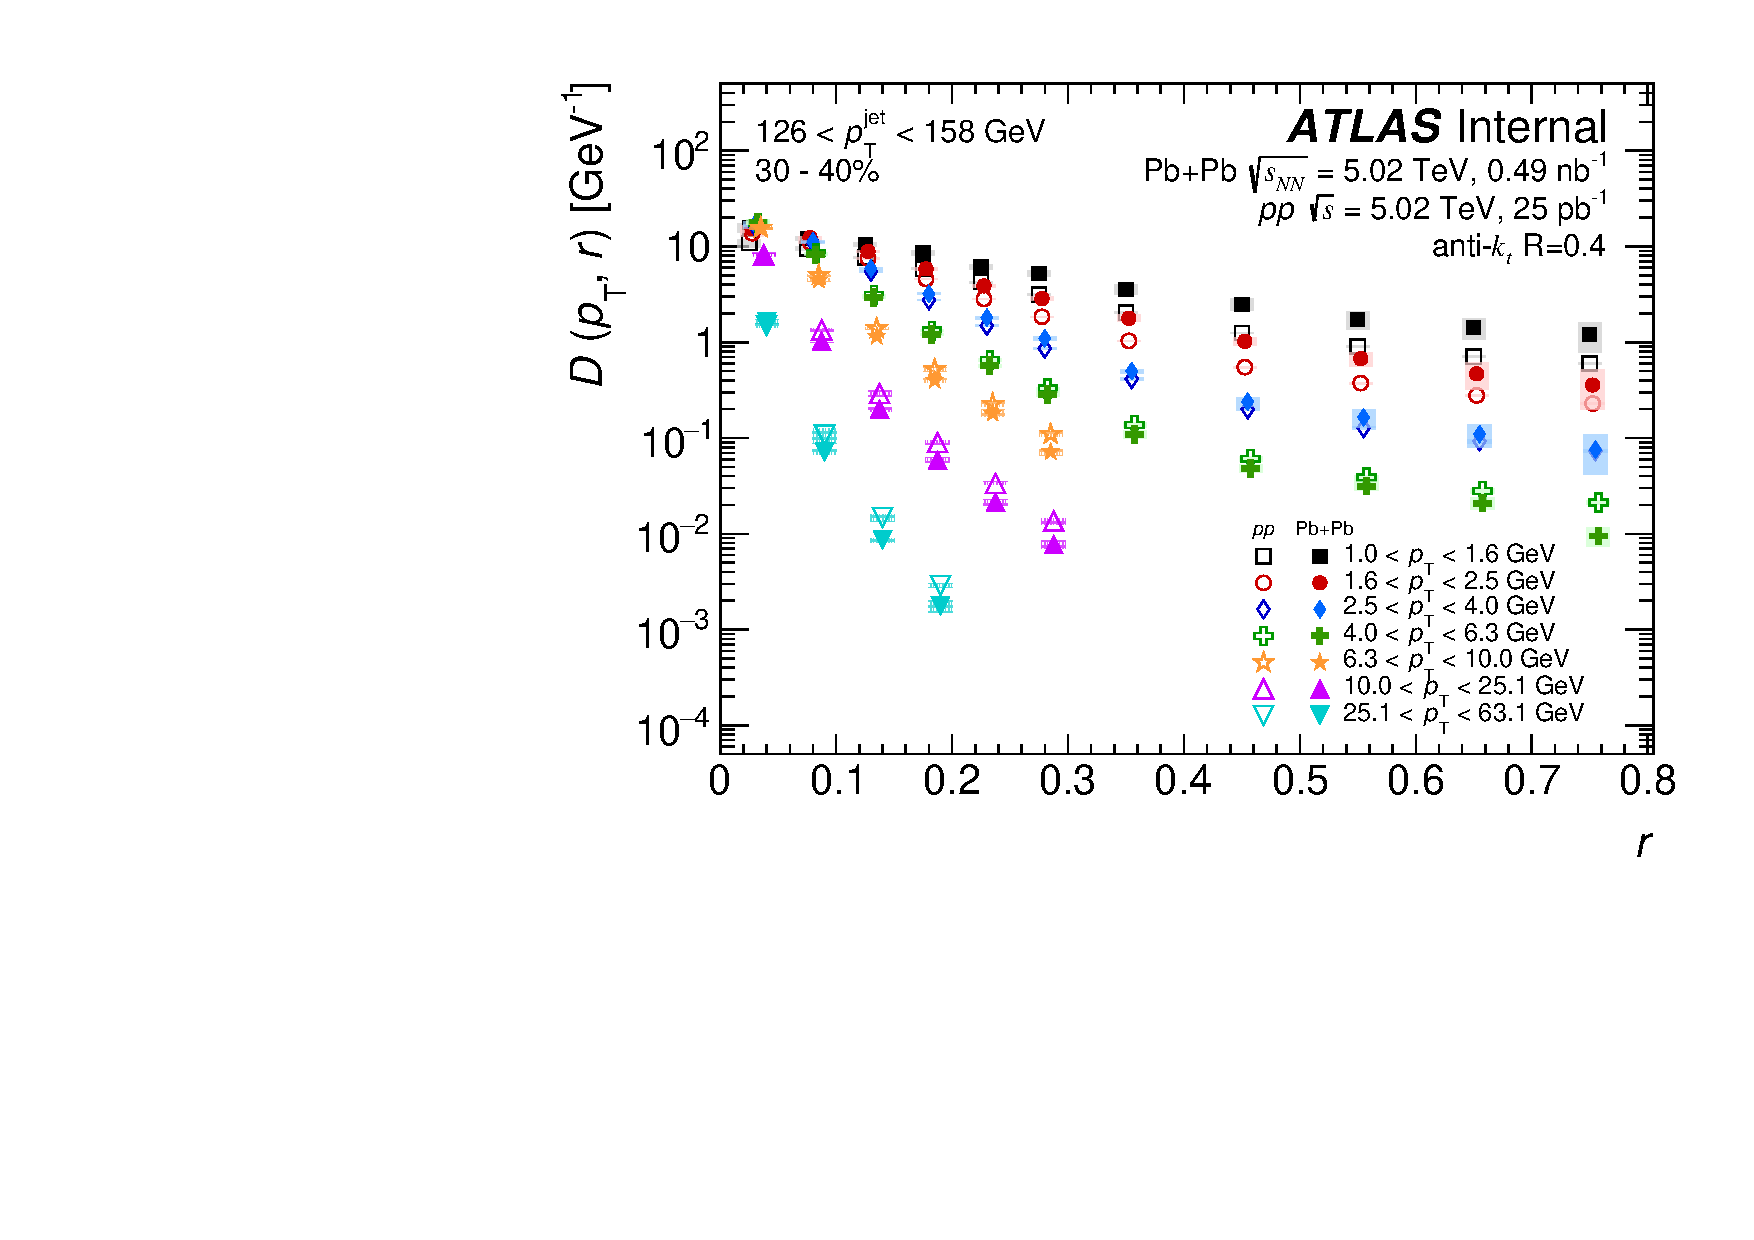
\includegraphics[width=0.36\textwidth]{figures/results/DpT_dR_jet7_cent3} &
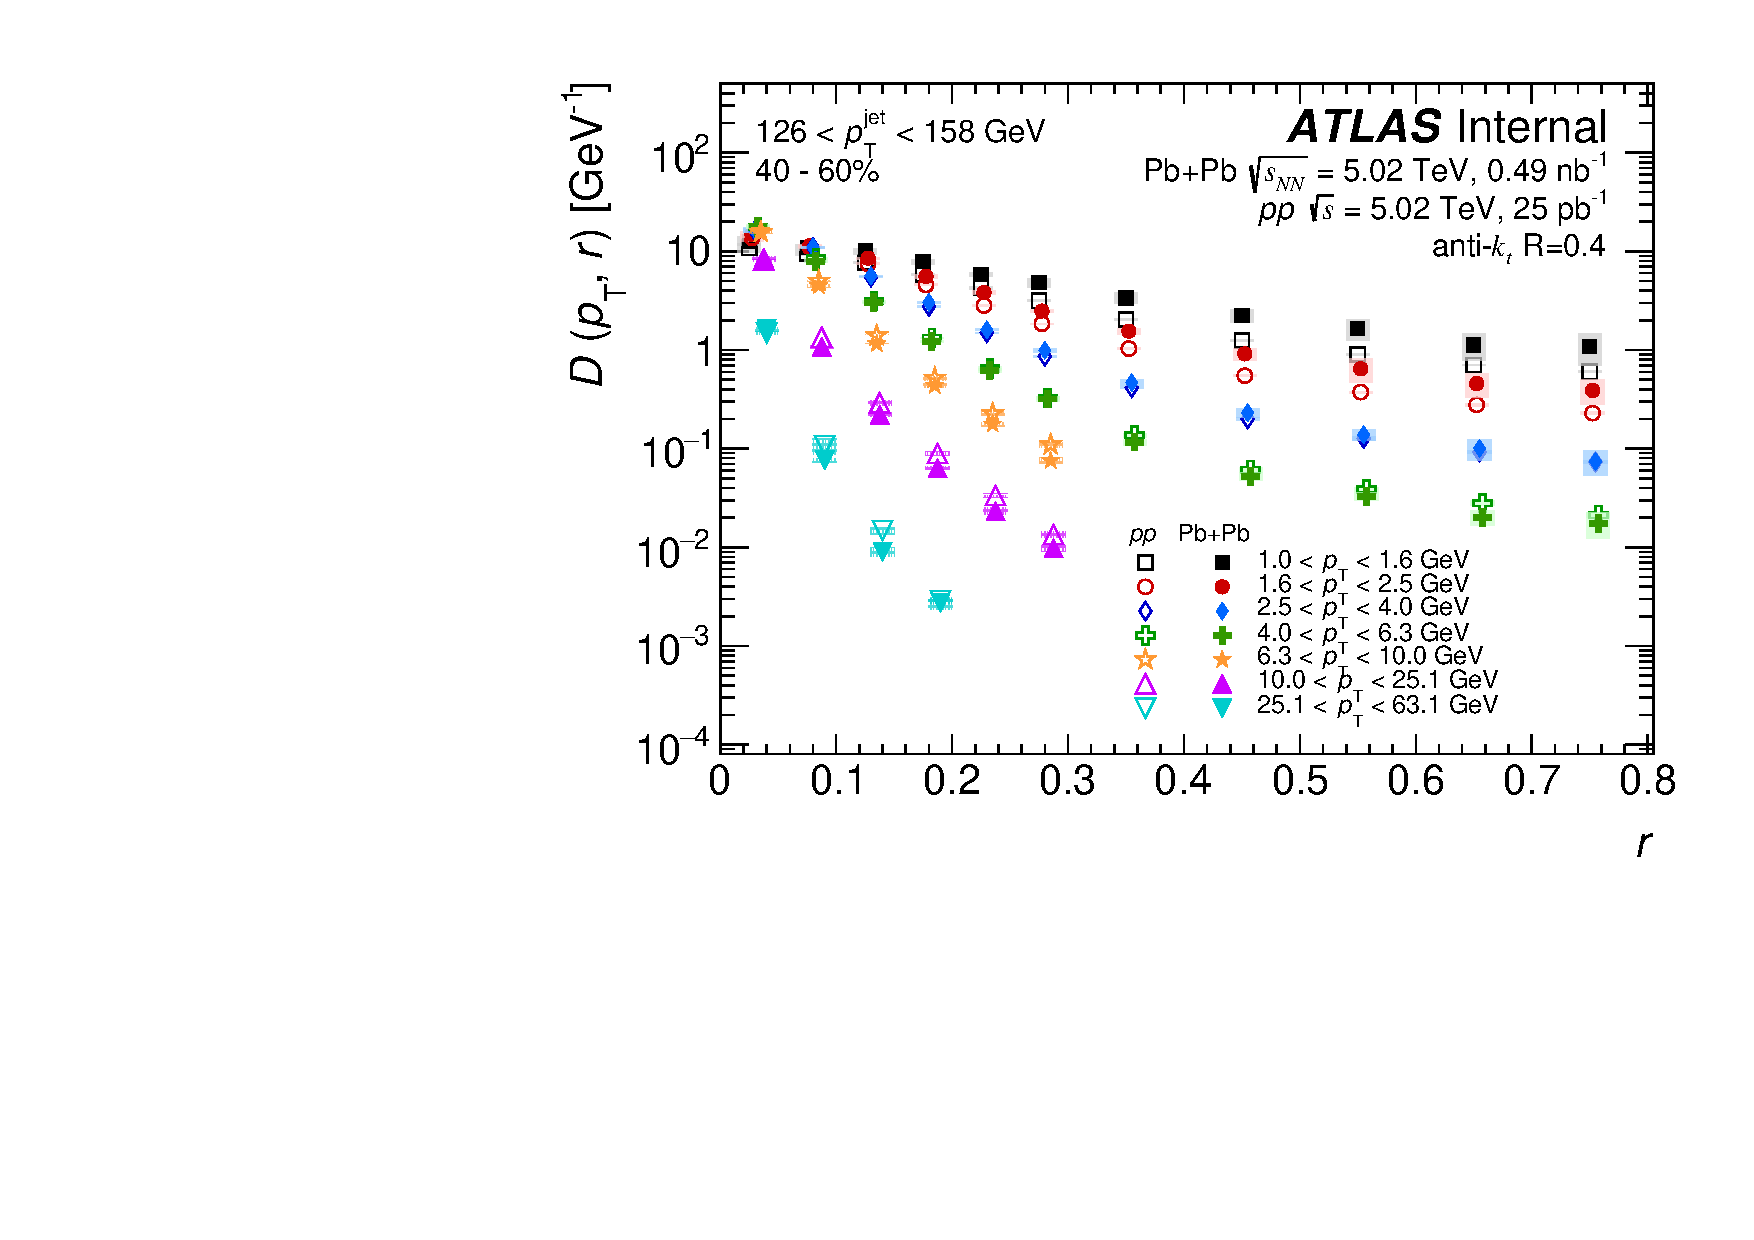
\includegraphics[width=0.36\textwidth]{figures/results/DpT_dR_jet7_cent4} &
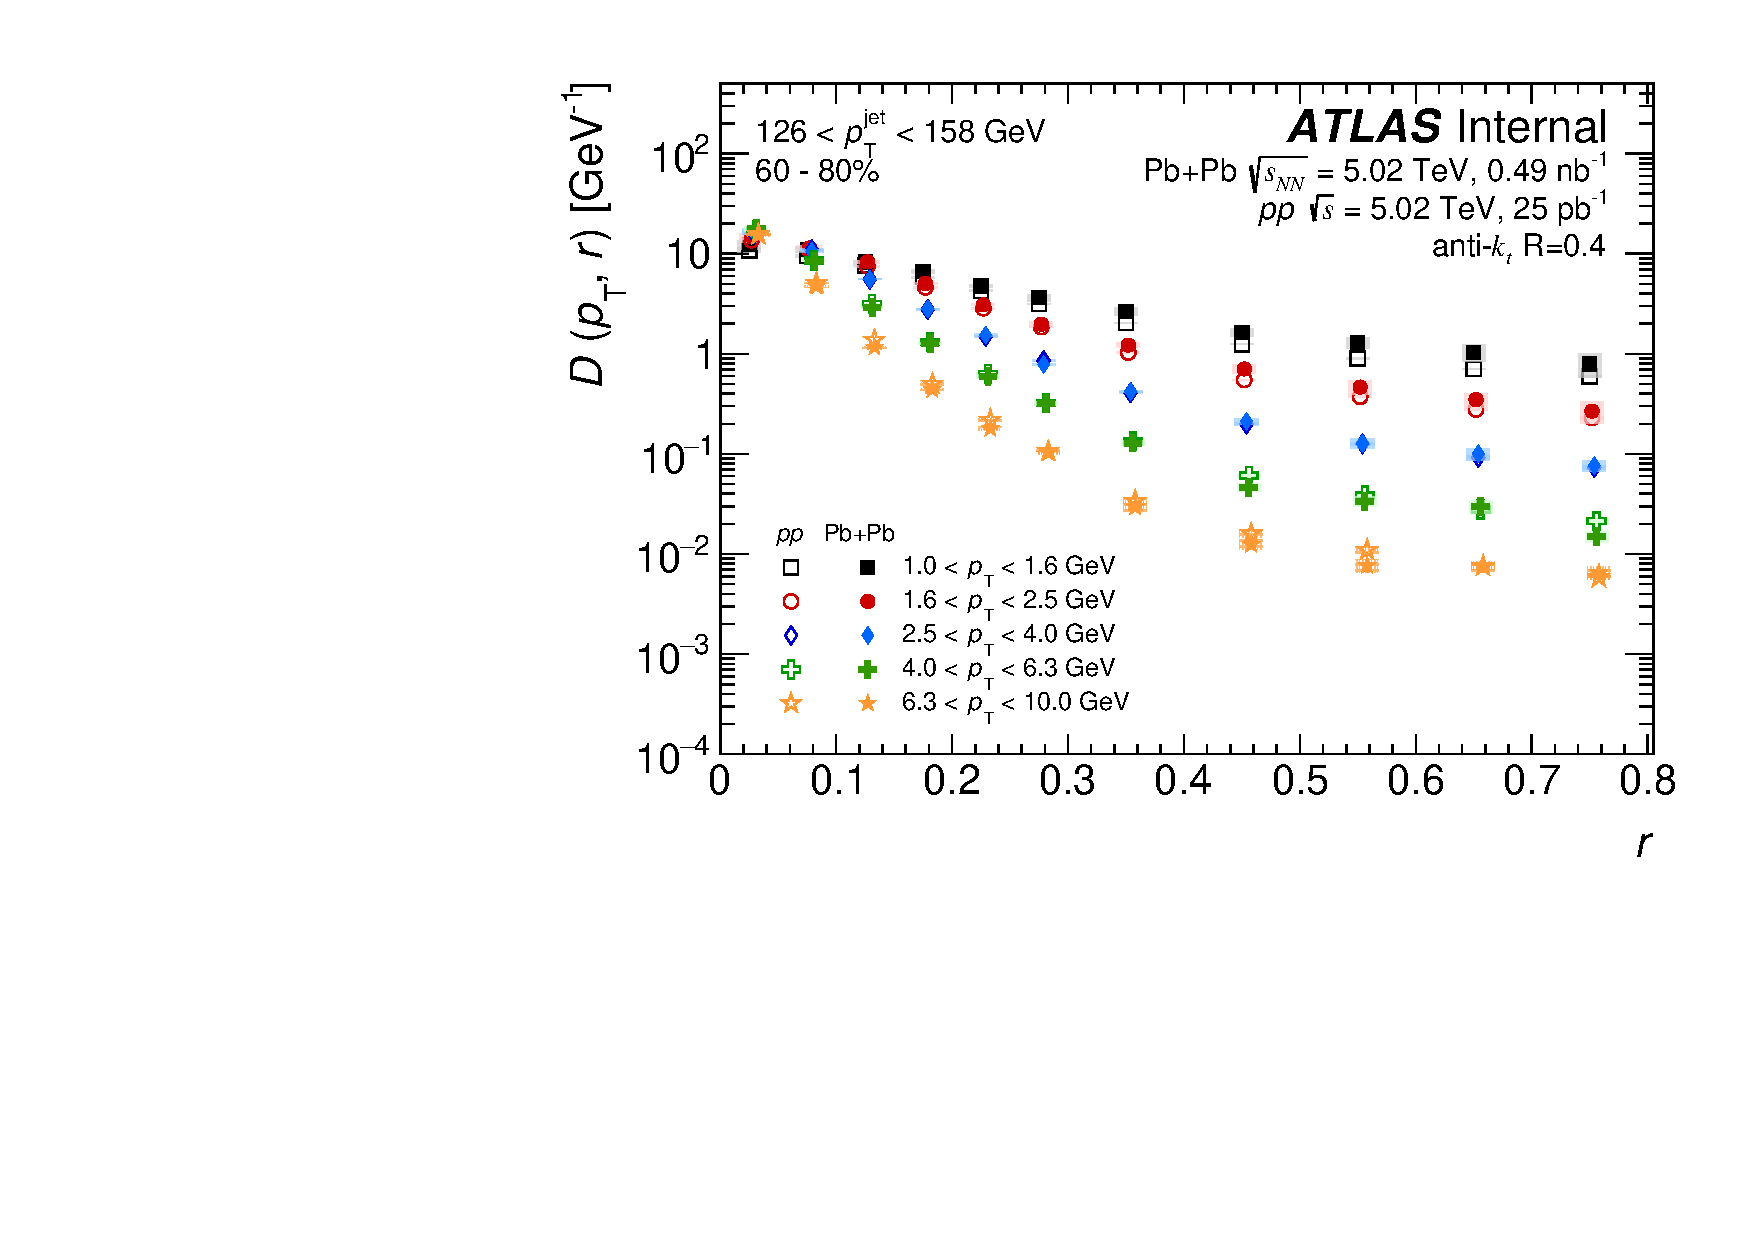
\includegraphics[width=0.36\textwidth]{figures/results/DpT_dR_jet7_cent5} \\
\end{tabular}
}
\caption{The \Dptr\ distributions in \pp\ (open symbols) and \pbpb\ (closed symbols) as a function of angular distance $r$ for \ptjet\ of 126 to 158~\GeV.
The colors represent different track \pt\ ranges, and each panel is a different centrality selection.
The vertical bars on the data points indicate statistical uncertainties while the shaded boxes indicate systematic uncertainties.
The widths of the boxes are not indicative of the bin size and the points are shifted horizontally for better visibility.
The distributions for $\pt > 6.3$ GeV are restricted to smaller \rvar\ values as discussed in Section~\ref{sec:analysis}.}
\label{fig:dptr}
\end{figure}



%%%%%%%    RDptr distributions    %%%%%%%
\subsection{\RDptr\ distributions}
\label{sec:rdptr}
In order to quantify the differences seen in Figure~\ref{fig:dptr}, ratios of the \Dptr\ distributions in \pbpb\ collisions to those measured in \pp\ collisions for $126 < \ptjet < 158$ GeV and $200 < \ptjet < 251$ GeV jets are presented in Figure~\ref{fig:rdptr}.
They are shown as a function of $r$ for different \pt\ and centrality selections.
In 0--10\% central collisions, \RDptr\ is greater than unity for $\rvar < 0.8$ for charged particles with \pT less than 4.0~\GeV\ in both jet selections.
For these particles, the enhancement of yields in \pbpb\ collisions compared to those in  \pp\ collisions grows with increasing \rvar\ up to approximately \mbox{$\rvar  = 0.3$}, with \RDptr\ reaching up to two for 1.0~$< \pt <$~2.5~\GeV.
The value of \RDptr\ is approximately constant for \rvar\ in the interval \mbox{0.3--0.6} and decreases for \mbox{$\rvar > 0.6$}.
For charged particles with $\pt > 4.0$ \GeV, \RDptr\ shows a depletion outside the jet core for $r > 0.05$.
The magnitude of this depletion increases with increasing \rvar\ up to $r = 0.3$ and is approximately constant thereafter.
The observed behavior inside the jet cone, $r < 0.4$, agrees with the measurement of the inclusive jet fragmentation functions~\cite{Aaboud:2017eww,Aaboud:2017bzv, Aaboud:2018hpb}, where yields of fragments with $\pt < 4$ GeV are observed to be enhanced and yields of charged particles with intermediate \pT\ are suppressed in \PbPb\ collisions compared to those in \pp\ collisions.
For 30--40\% mid-central collisions, the enhancement of particles with $\pt < 4.0$~\GeV\ is similar to that in the most central collisions, however the depletion of particles with $\pt > 4.0$~\GeV\ is not as strong.
For 60--80\% peripheral collisions, \RDptr\ has no significant \rvar\ dependence and the values of \RDptr\ are within approximately 50\% of unity.
The variation of \RDptr\ with centrality, \ptjet, and charged-particle \pt\ is further discussed.

\begin{figure}[h]
\centerline{
\begin{tabular}{ccc}
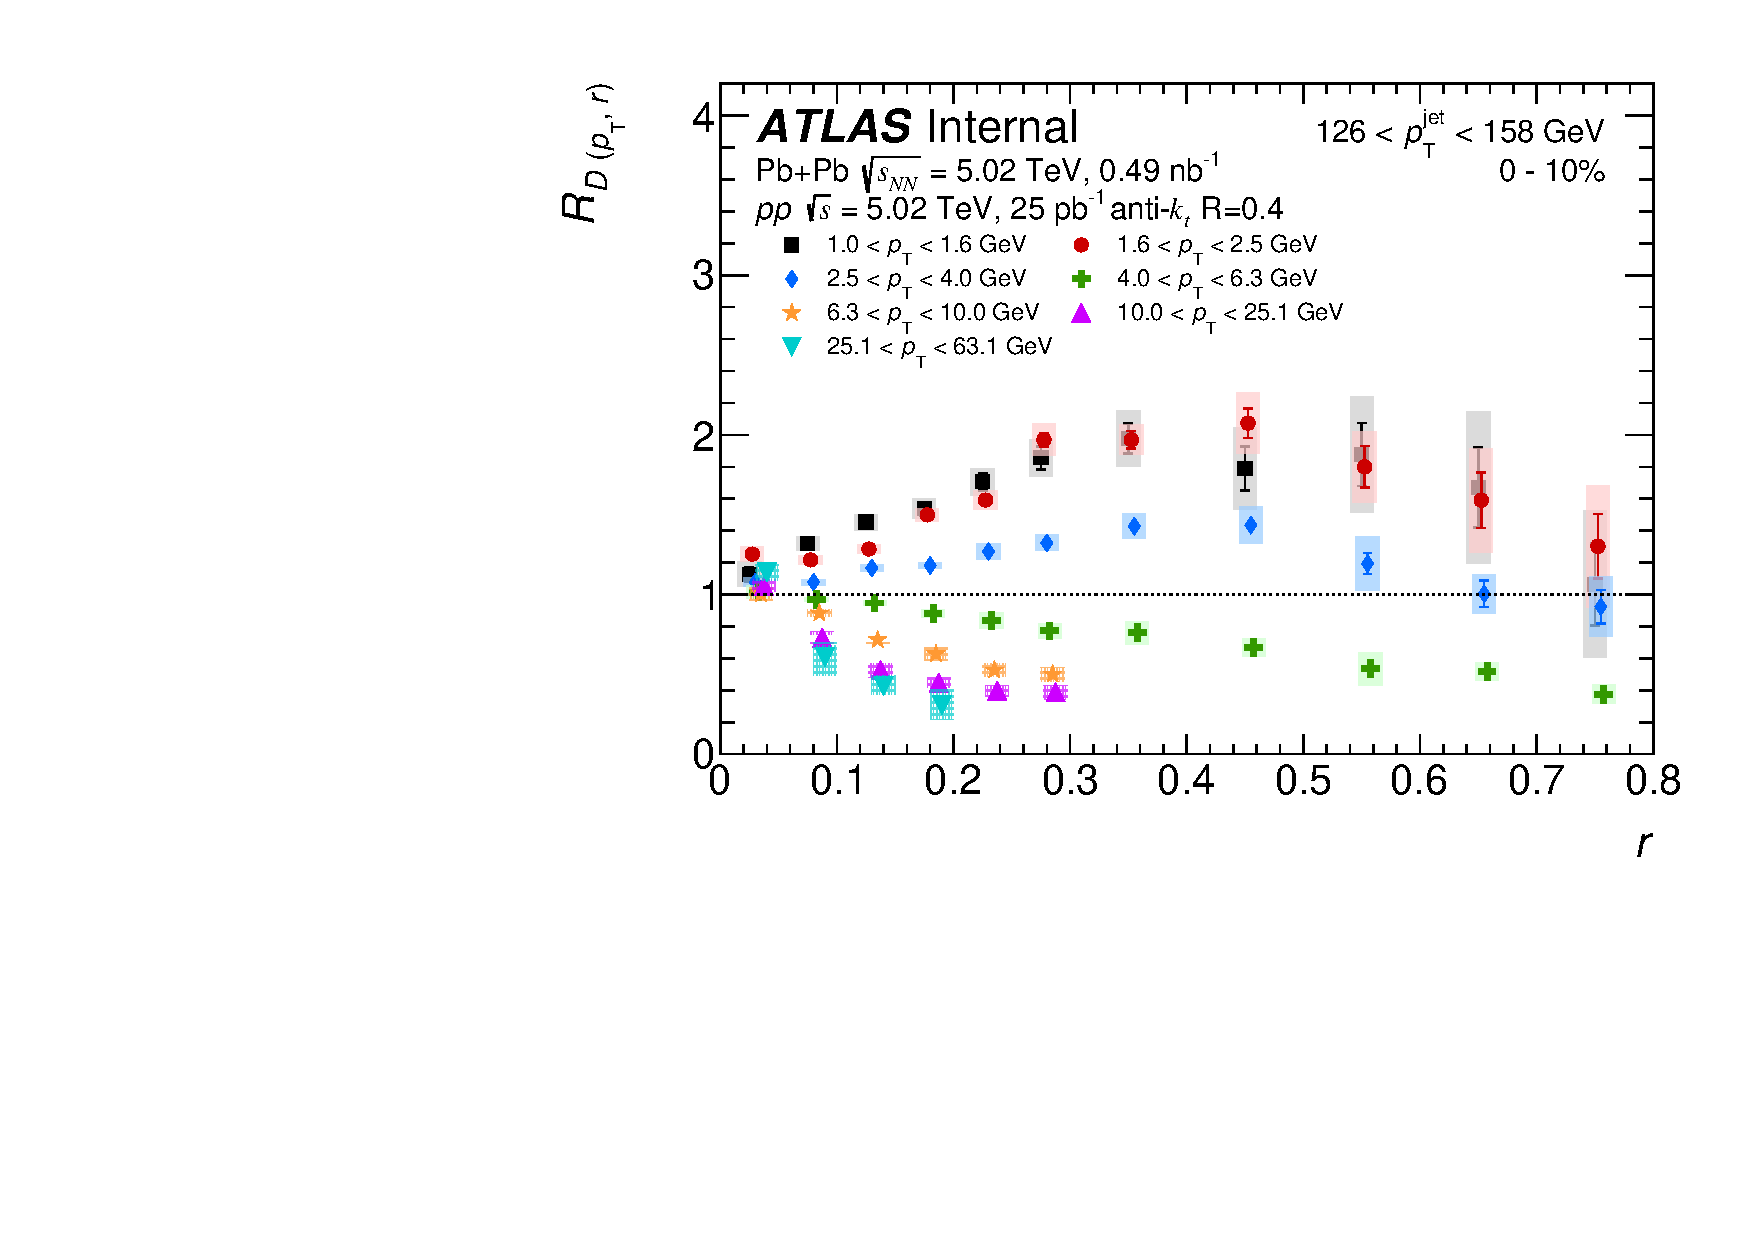
\includegraphics[width=0.36\textwidth]{figures/results/RDpT_dR_jet7_cent0} &
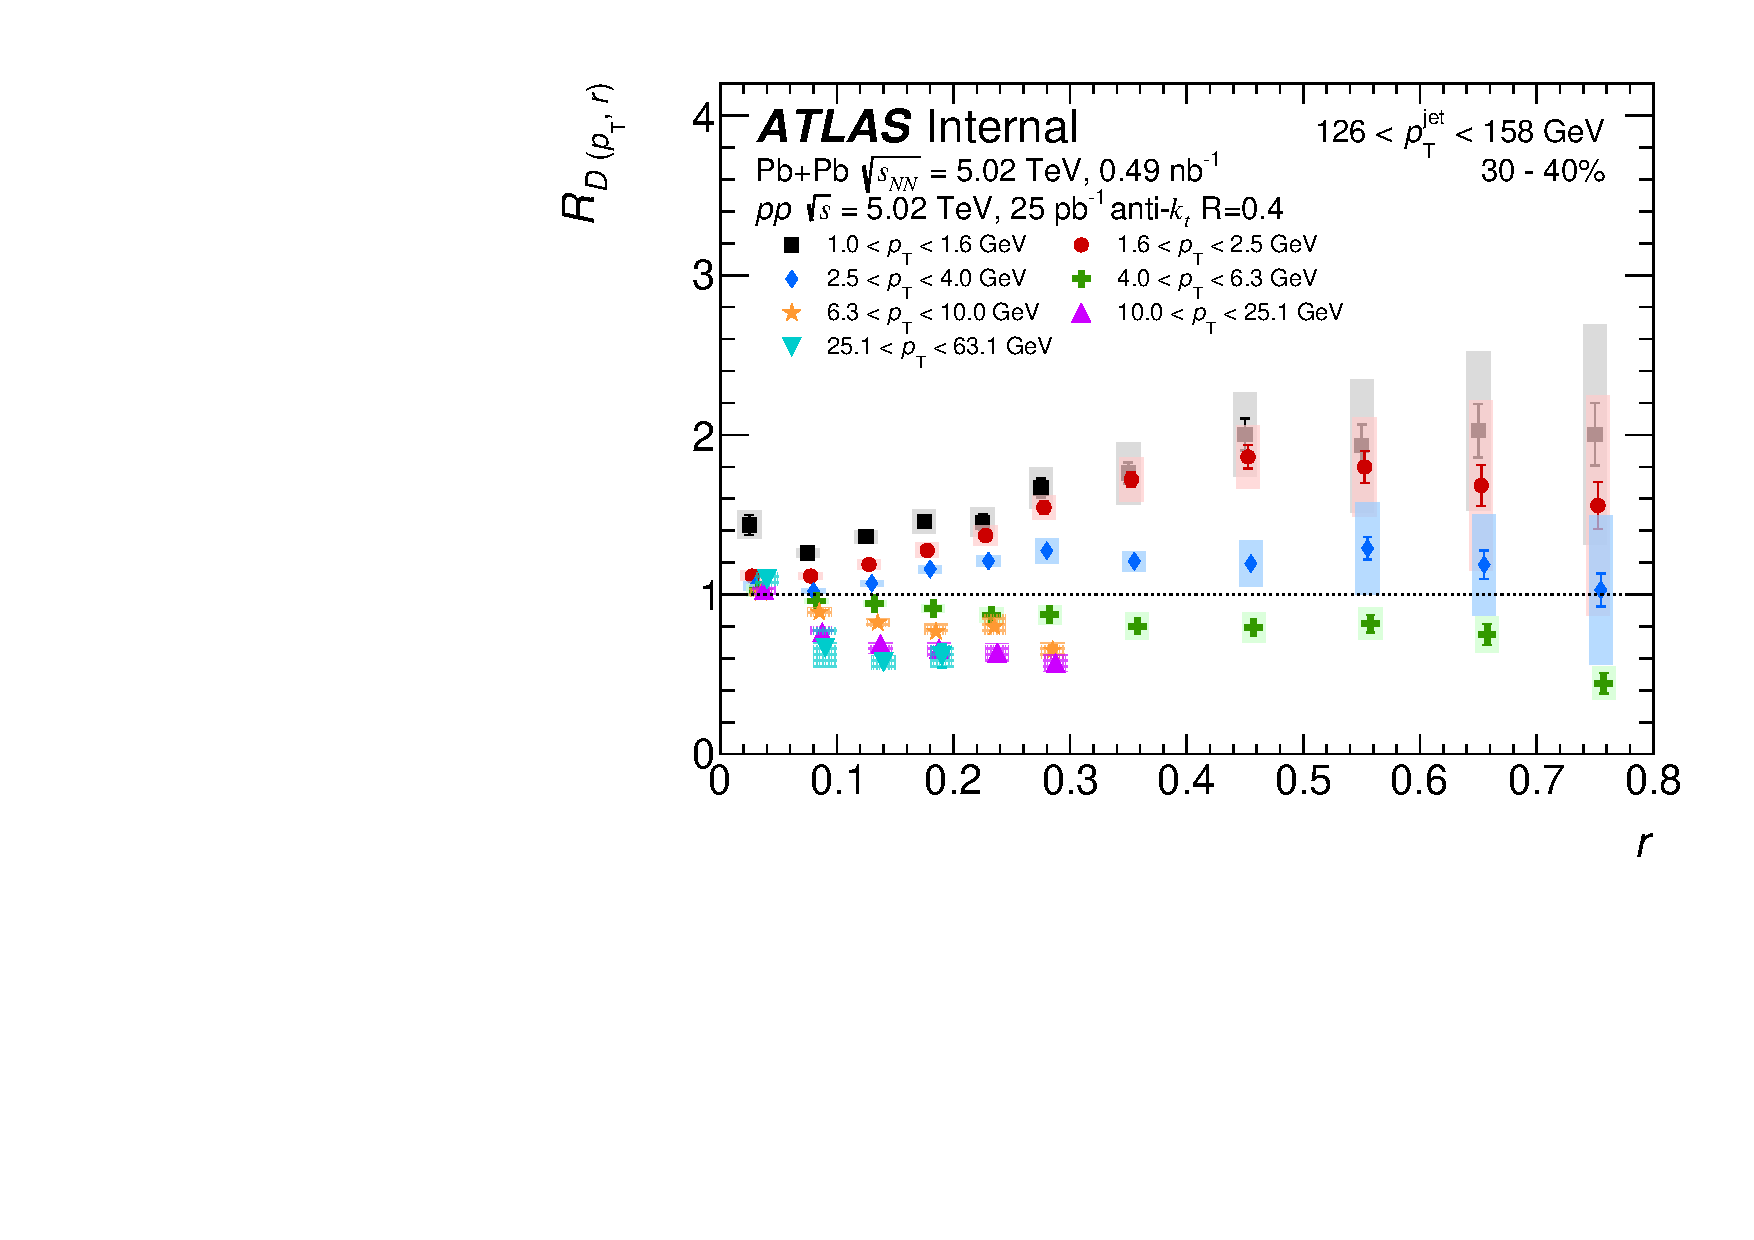
\includegraphics[width=0.36\textwidth]{figures/results/RDpT_dR_jet7_cent3} &
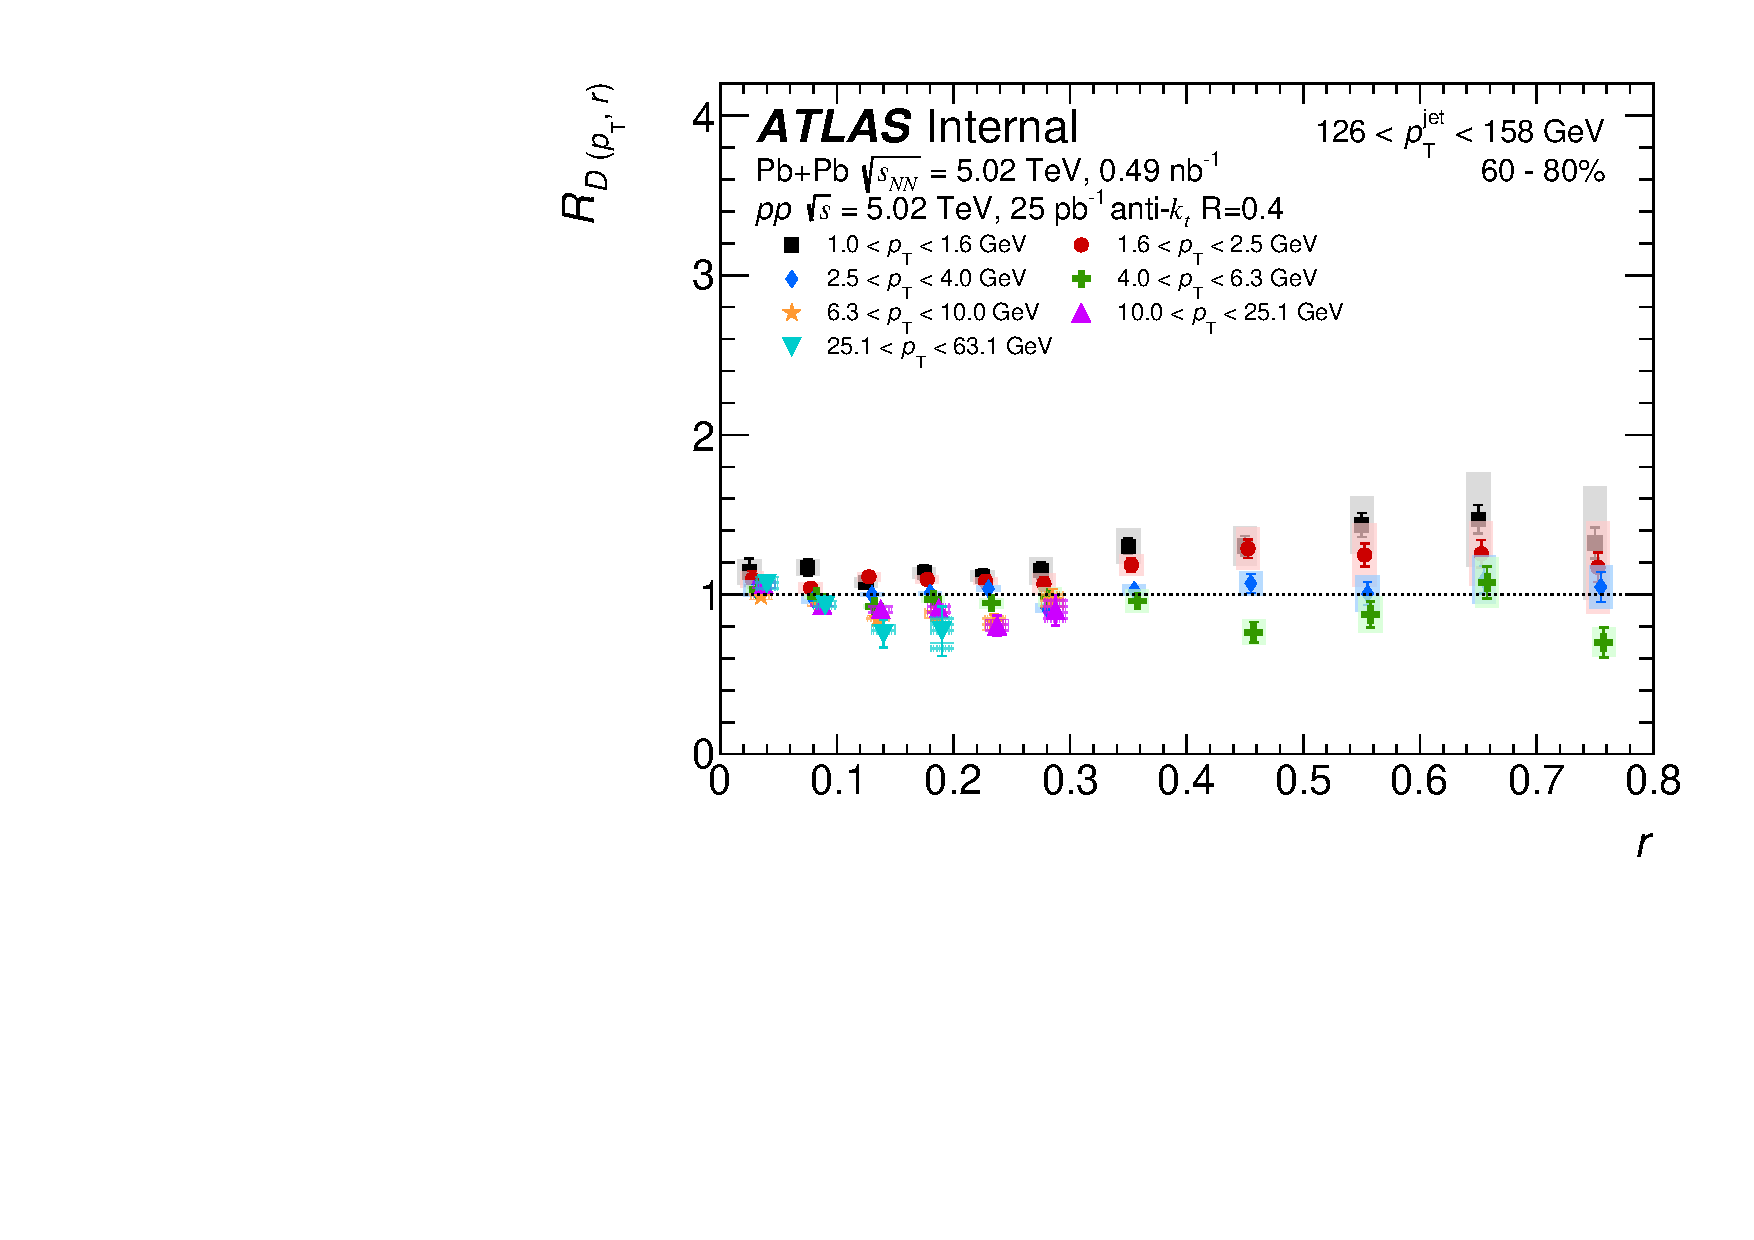
\includegraphics[width=0.36\textwidth]{figures/results/RDpT_dR_jet7_cent5} \\
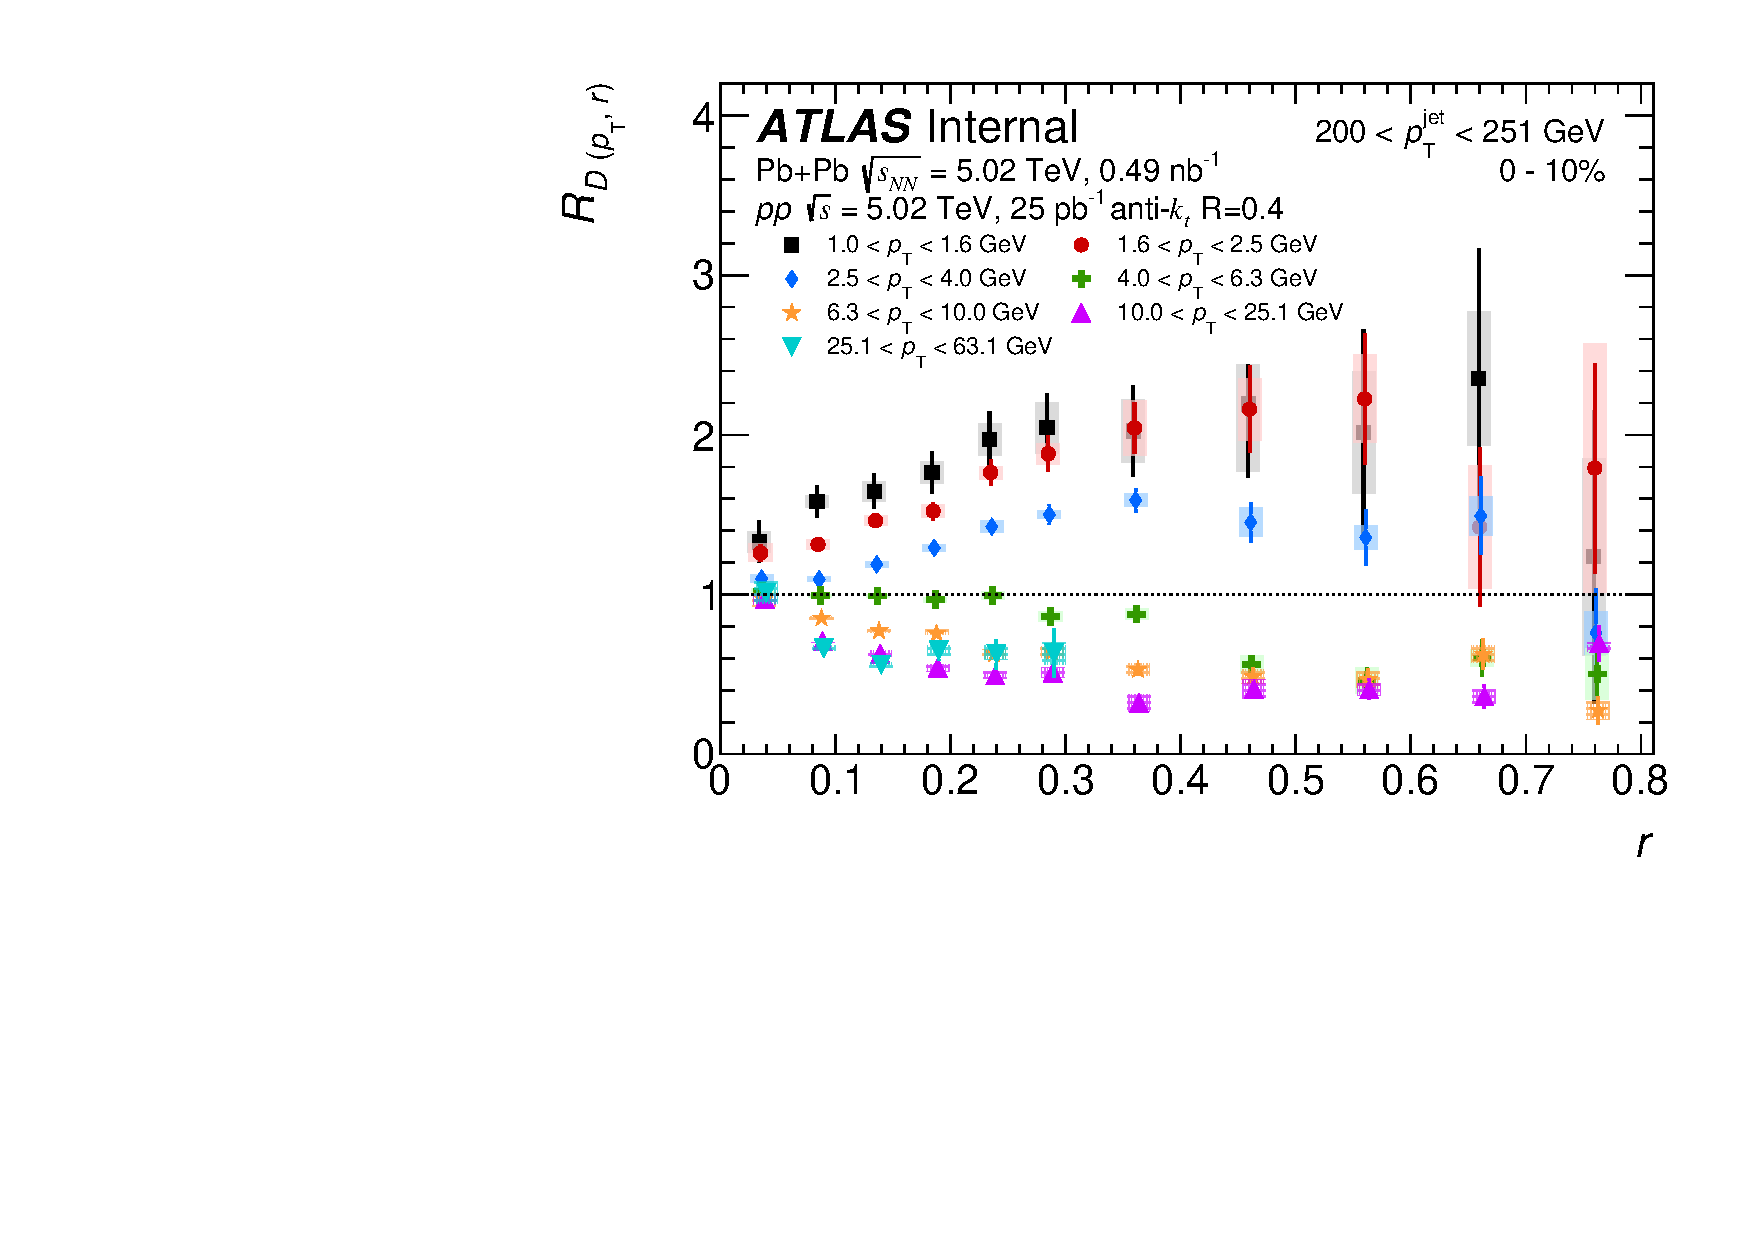
\includegraphics[width=0.36\textwidth]{figures/results/RDpT_dR_jet9_cent0} &
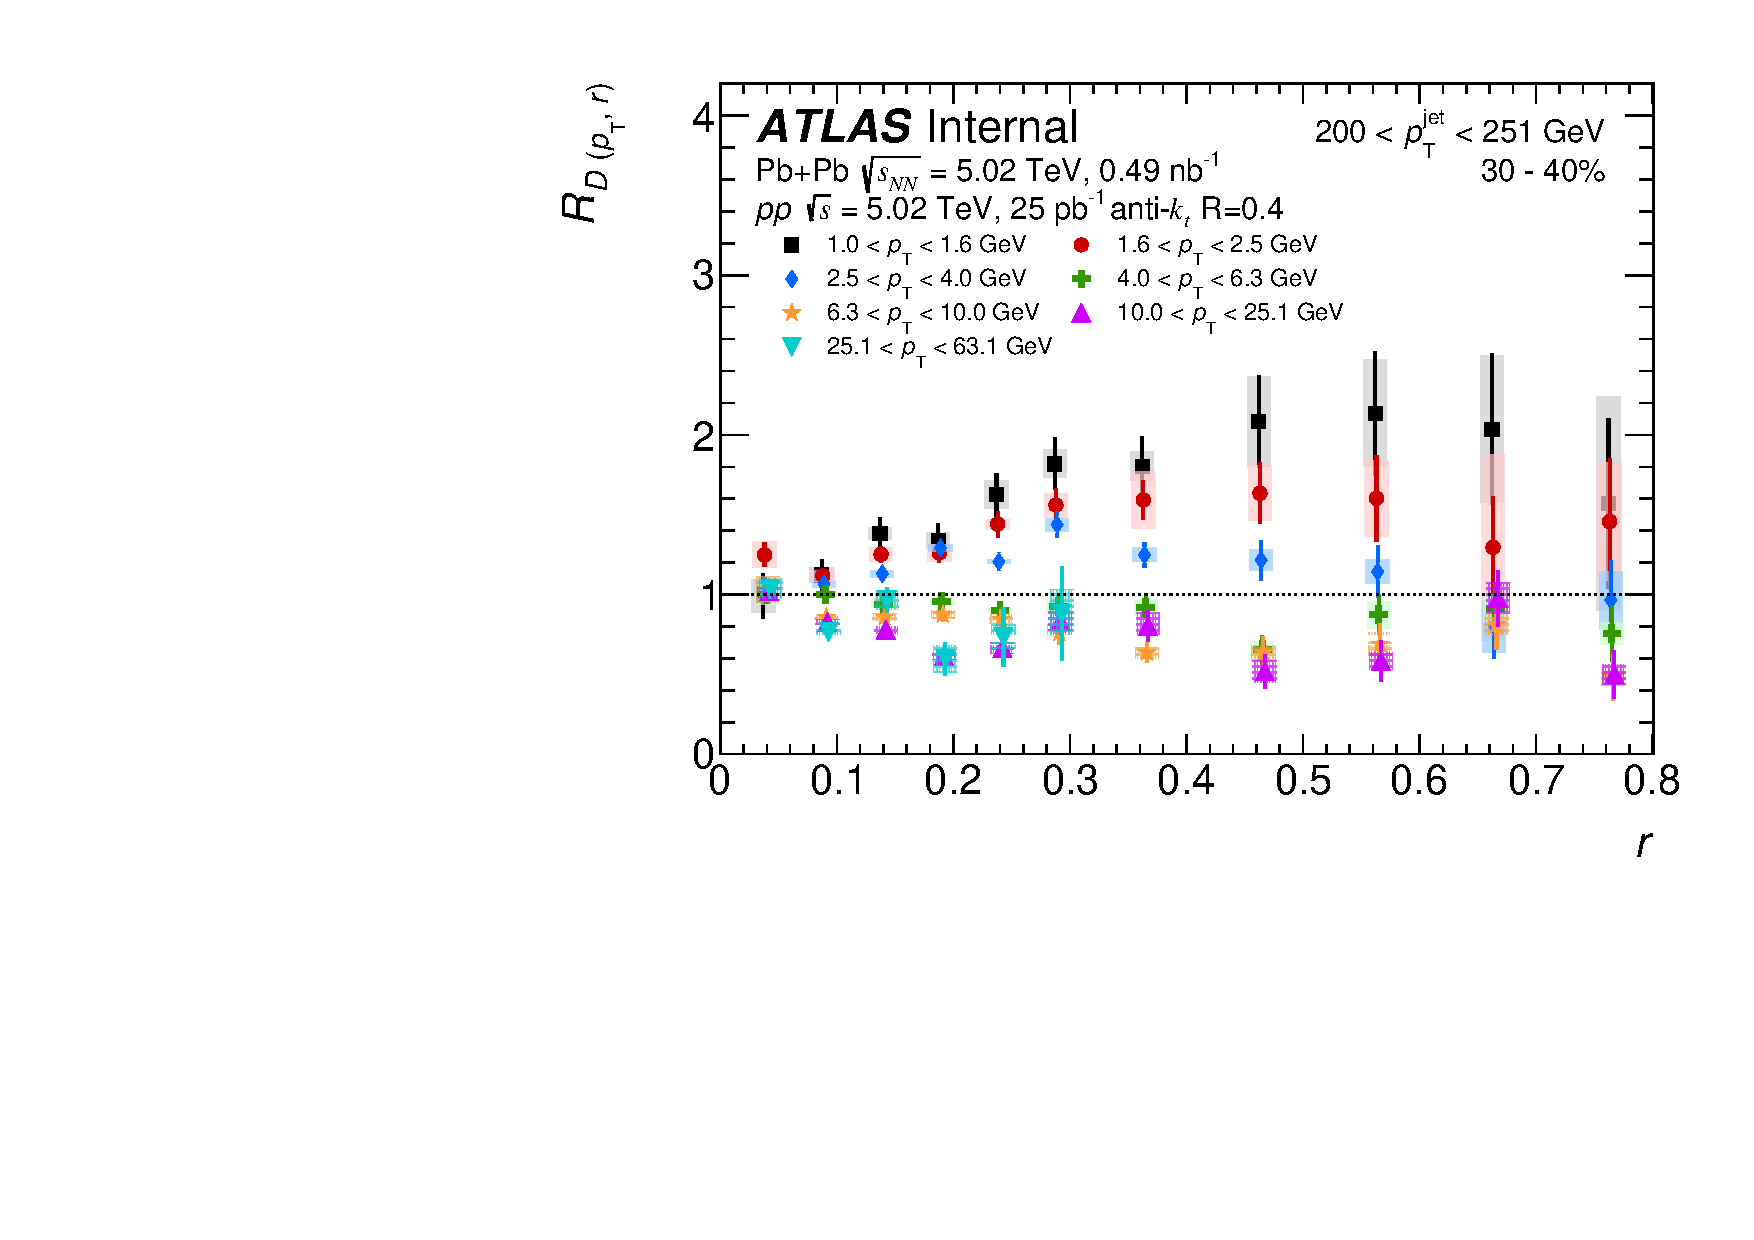
\includegraphics[width=0.36\textwidth]{figures/results/RDpT_dR_jet9_cent3} &
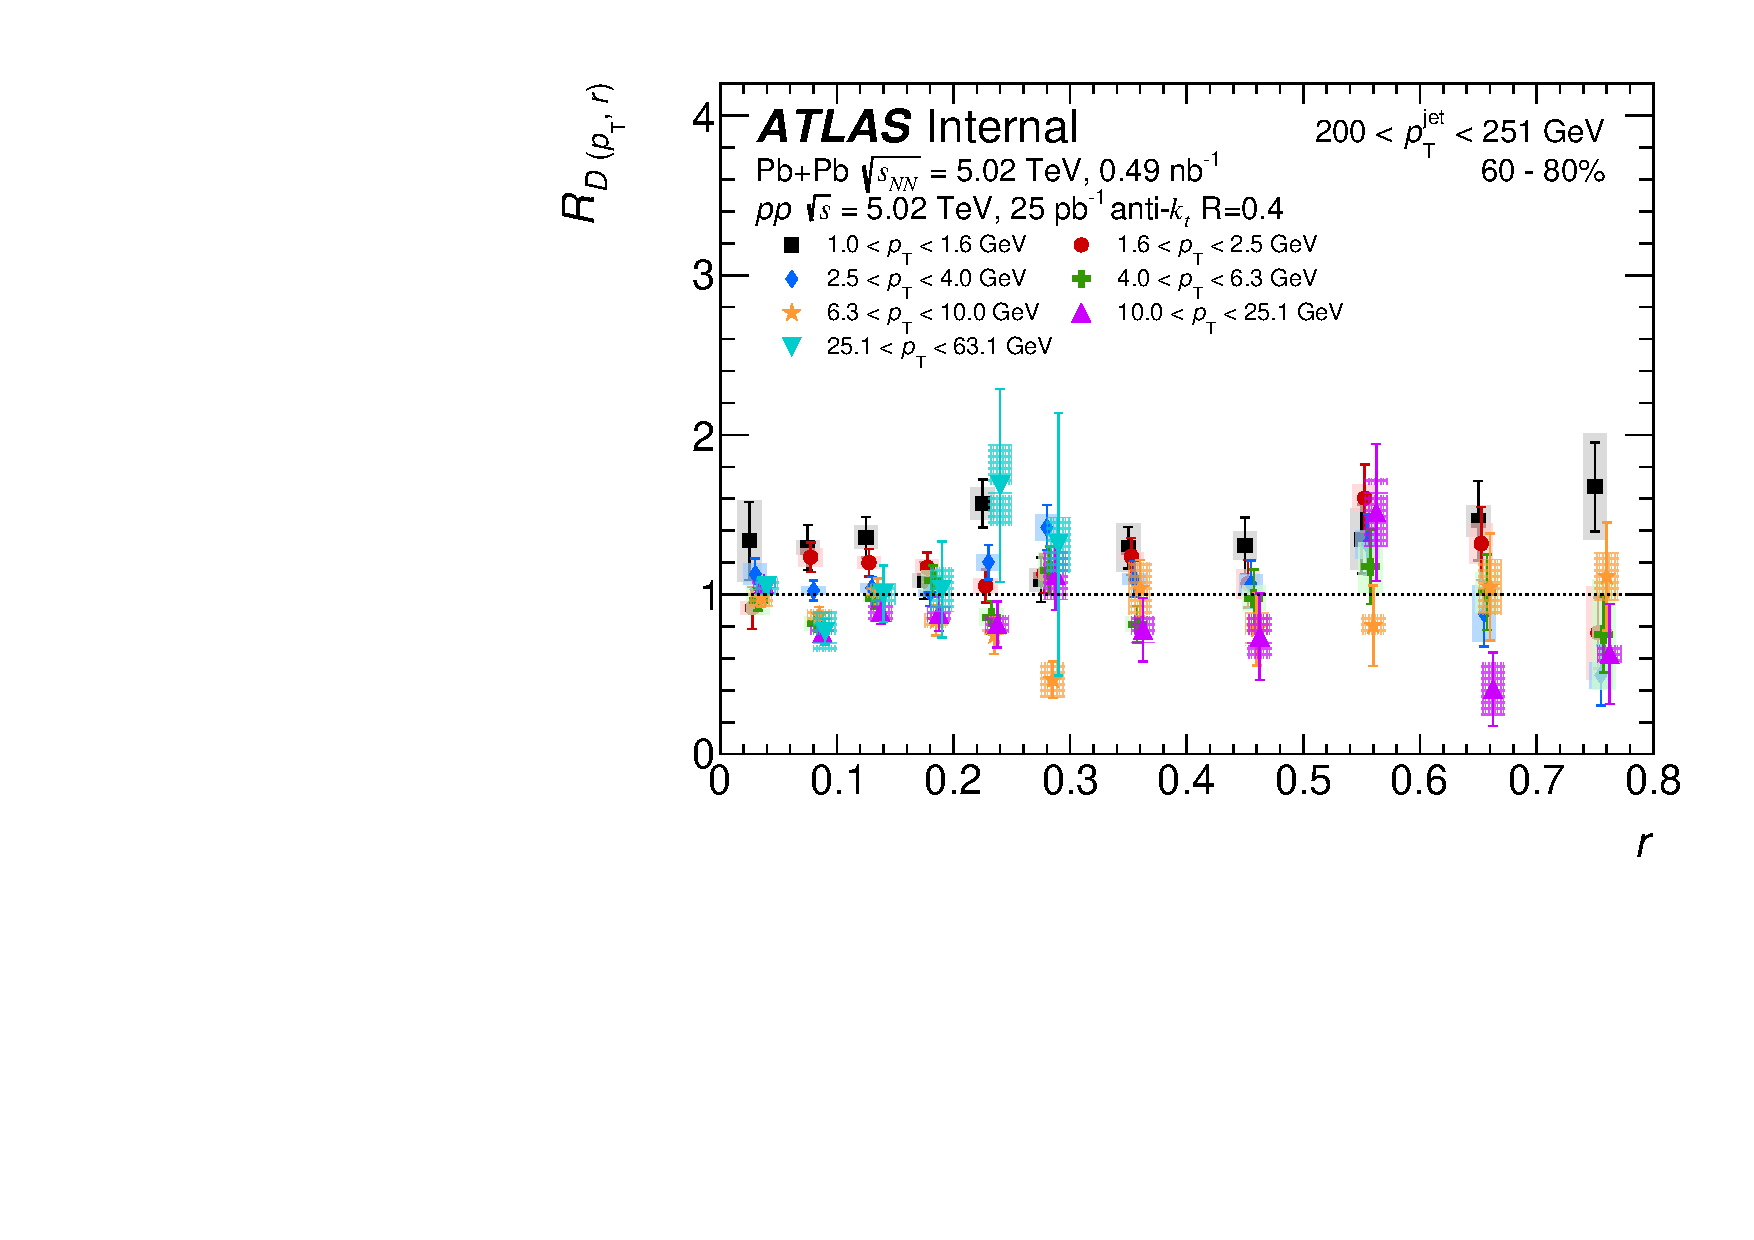
\includegraphics[width=0.36\textwidth]{figures/results/RDpT_dR_jet9_cent5} \\
\end{tabular}
}
\caption{Ratios of \Dptr\ distributions in \PbPb\ and \pp\ collisions as a function of angular distance $r$ for \ptjet\ of 126 to 158~\GeV\ (top) and of 200 to 251~\GeV\ (bottom) for seven \pt\ selections.
Different centrality selections are shown: 0--10\% (left), 30--40\% (middle), 60--80\% (right).
The vertical bars on the data points indicate statistical uncertainties while the shaded boxes indicate systematic uncertainties.
The widths of the boxes are not indicative of the bin size and the points are shifted horizontally for better visibility.}
\label{fig:rdptr}
\end{figure}

% This observation is in agreement with the previous measurement of jet fragmentation functions \cite{Chatrchyan:2014ava, Sirunyan:2018jqr, Aaboud:2017bzv, } and may indicate the dependence of the response of the hot dense matter to the momentum of a jet passing through it.
%\FloatBarrier
